\section{Supplementary Experiments on Proximal and Distal Distillation}
\label{app:distillation-experiments}

We provide the experimental settings and additional results for the
distillation comparison in the main body. The experiments consider three
settings: a teacher identical to the initial student, teachers obtained
by briefly training the initial student with GRPO, and an existing strong
teacher applied to students with different initial capabilities. These
settings allow us to examine the proximal-limit prediction and the
behavior of distillation beyond this limit.

\subsection{Experimental settings}

\paragraph{Distillation objectives.}
Let $\pi_\theta$ be the student and $\pi_t$ a frozen teacher. Following
the main body, the two population objectives to maximize are
\begin{align}
 \mathcal J_{\mathrm{KD}}(\theta)
 &=-\mathbb E_{x\sim\mathcal D}
 D_{\mathrm{KL}}\bigl(\pi_t(\cdot\mid x)\Vert
                       \pi_\theta(\cdot\mid x)\bigr),
 \label{eq:app-distillation-kd}\\
 \mathcal J_{\mathrm{OPD}}(\theta)
 &=-\mathbb E_{x\sim\mathcal D}
 D_{\mathrm{KL}}\bigl(\pi_\theta(\cdot\mid x)\Vert
                       \pi_t(\cdot\mid x)\bigr).
 \label{eq:app-distillation-opd}
\end{align}
Sampled-response KD approximates the teacher expectation using a fixed
cache $\mathcal C_t$ of prompt--response pairs. Its empirical loss is
\begin{equation}
 \widehat{\mathcal L}_{\mathrm{SFT}}(\theta)
 =-\frac{1}{|\mathcal C_t|}\sum_{(x,y)\in\mathcal C_t}
   \sum_{k=1}^{|y|}\log\pi_\theta(y_k\mid x,y_{<k}).
 \label{eq:app-distillation-sft-loss}
\end{equation}
This is the SFT implementation of KD referred to in the figures and
tables. OPD instead samples from the current student and obtains
teacher log-probabilities on the student's prefixes. Writing
\begin{equation}
 w_\theta(y\mid x)
 =\log\frac{\pi_t(y\mid x)}{\pi_\theta(y\mid x)}
 =\sum_{k=1}^{|y|}\log
   \frac{\pi_t(y_k\mid x,y_{<k})}{\pi_\theta(y_k\mid x,y_{<k})},
 \label{eq:app-distillation-log-ratio}
\end{equation}
the corresponding population gradient is
\begin{equation}
 \nabla_\theta\mathcal J_{\mathrm{OPD}}
 =\mathbb E_{x\sim\mathcal D,\,y\sim\pi_\theta(\cdot\mid x)}
 \left[w_\theta(y\mid x)\nabla_\theta\log\pi_\theta(y\mid x)\right].
 \label{eq:app-distillation-opd-gradient}
\end{equation}
The sampled responses and log-ratio weights are detached in the score
update, as in Appendix~\ref{app:proximal-gradient-noise}. Thus both
methods match the same teacher distribution, but use different sampling
distributions and gradient weights. Task rewards only monitor response
correctness and do not contribute to either distillation objective.

\paragraph{Models and training.}
For the proximal-limit experiment, we initialize both the student and
the frozen teacher from Qwen3-1.7B-Base. For the proximal experiments,
we use the same initial student and three GRPO-trained teachers,
denoted GRPO-50, GRPO-100, and GRPO-200. For the remaining experiments,
we use a JustRL teacher with R1-Distill-1.5B and Qwen2.5-Math-1.5B
students. Both students use the same cached teacher responses for SFT.
The latter pair has a larger initial benchmark performance gap.

Training uses the slime framework with Megatron and SGLang, at revision
\texttt{a067ce6f}. The Qwen3 experiments use DAPO17k, a maximum response
length of 2,048 tokens. The JustRL experiments use the JustRL training
data and a maximum response length of 8,192 tokens. Runs use seed 1.
The proximal-limit runs use a learning rate of $10^{-5}$.

\paragraph{Evaluation and interpretation of the curves.}
Each evaluation samples 16 responses per problem at temperature 1,
with a maximum response length of 16,384 tokens, and uses the
DAPO/math-verify grader. Scores are average correctness over sampled
responses, expressed as percentages. We evaluate on AIME-2024, AMC23,
and MATH500 and report their unweighted mean.

The reward curves have different meanings for the two methods. For
OPD, they measure correctness of responses generated by the evolving
student. For SFT, they measure correctness of the cached teacher
responses in each batch. The SFT curves can therefore fluctuate with
batch composition even though the response cache is fixed. Their level
does not measure the trained student's performance. We use the separate
held-out evaluations for comparisons between the two methods.
The recorded Qwen3 base reference uses a shorter evaluation limit of
4,096 tokens.

\subsection{Behavior at the proximal limit}

Figure~\ref{fig:distillation-proximal-limit} shows gradient norms when
the frozen teacher initially coincides with the student. In addition to
offline SFT on a fixed self-generated cache, we include online SFT,
which refreshes responses from the current student, and controls that
reverse the update direction. In the legend, ``fwd'' and ``rev'' denote
the ordinary and sign-reversed updates, respectively; they do not denote
the two directions of KL divergence.

\begin{figure}[htbp]
\centering
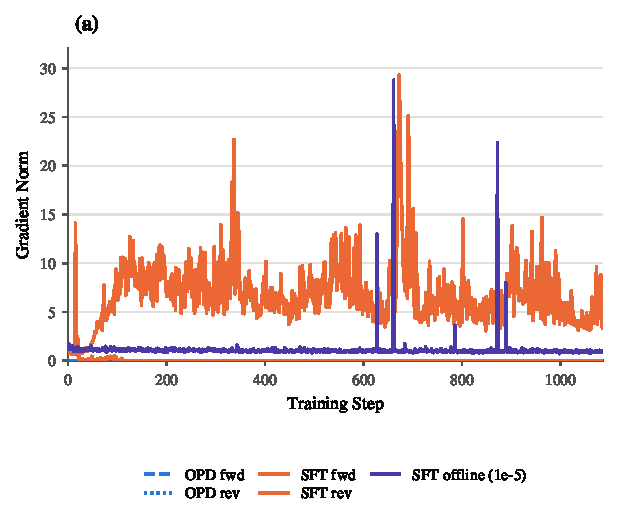
\includegraphics[width=0.68\linewidth]{media/selfdist_gradnorm.pdf}
\caption{Gradient norms with Qwen3-1.7B-Base as both the initial student
and the frozen teacher. Both OPD directions have zero recorded gradient
norm throughout training, with their traces overlapping at zero.
The SFT runs exhibit nonzero sampled gradients. Offline SFT uses a
fixed cache, whereas the other SFT controls regenerate responses from
the evolving student. All runs use a learning rate of $10^{-5}$.}
\label{fig:distillation-proximal-limit}
\end{figure}

Both OPD runs have exactly zero recorded gradient norm throughout
training. This agrees with Lemma~\ref{lem:proximal-gradient-noise}:
the sampled log-ratio weight vanishes when teacher and student coincide,
so reversing its sign also leaves the update zero. SFT exhibits nonzero
sampled gradients even at initialization, as expected for sampled-response
cross-entropy. Offline SFT subsequently fits the finite response cache,
while online SFT also changes its sampling distribution as training
proceeds. Thus the initial contrast illustrates the proximal-limit
prediction; the later SFT trajectory is no longer a measurement at that
limit. In particular, a training gradient norm is not a direct estimate
of gradient variance at fixed parameters.

\begin{takeaway}
At the proximal limit, both distillation objectives have zero population
gradient, but their sampled updates behave differently: OPD vanishes
samplewise while sampled-response KD retains gradient noise. This
illustrates the gradient-estimation distinction underlying the proximal
advantage discussed in the main body.
\end{takeaway}
\FloatBarrier

\subsection{Distillation from nearby teachers}

Figure~\ref{fig:distillation-proximal} shows training with the three
GRPO teachers. Student rollout correctness under OPD quickly
approaches the range of the corresponding teacher-cache correctness.
The evaluations in Table~\ref{tab:distillation-performance}
provide the student-to-student comparison. OPD attains
mean scores of 17.77, 20.75, and 26.63 for GRPO-50, GRPO-100, and
GRPO-200, compared with 16.78, 19.81, and 26.07 for SFT.
These observations are consistent with a local advantage of
OPD, although the single-seed results do not establish statistical
significance or directly test the gradient-variance ordering.
%
% \begin{figure}[htbp]
% \centering
% 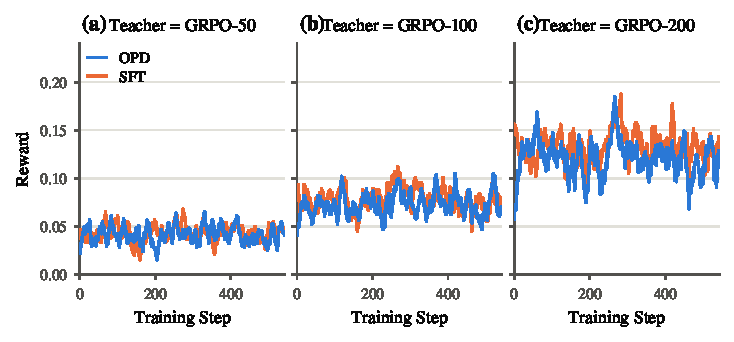
\includegraphics[width=\linewidth]{media/selfdist_proximal.pdf}
% \caption{Distillation from the three GRPO-trained Qwen3 teachers.
% OPD rewards measure current student rollout correctness; SFT rewards
% measure cached teacher-response correctness, rather than SFT student
% performance. Each panel uses Qwen3-1.7B-Base as the initial student.}
% \label{fig:distillation-proximal}
% \end{figure}

\FloatBarrier

\subsection{Distillation with a larger initial performance gap}

Figure~\ref{fig:distillation-distal} compares two students trained
with the JustRL teacher. The R1-Distill-1.5B student starts at a mean
benchmark score of 53.56, compared with 72.27 for the teacher. Both
methods reach scores close to the teacher: SFT and OPD scores
are 72.94 and 72.04, respectively. Under this setting both algorithms remain stable, while SFT is already slightly more performant.

The Qwen2.5-Math-1.5B student starts substantially lower, at 15.27.
Its OPD rollout correctness decreases early and remains low over the
displayed interval, whereas SFT reaches an evaluation score of
47.46.

\begin{figure}[htbp]
\centering
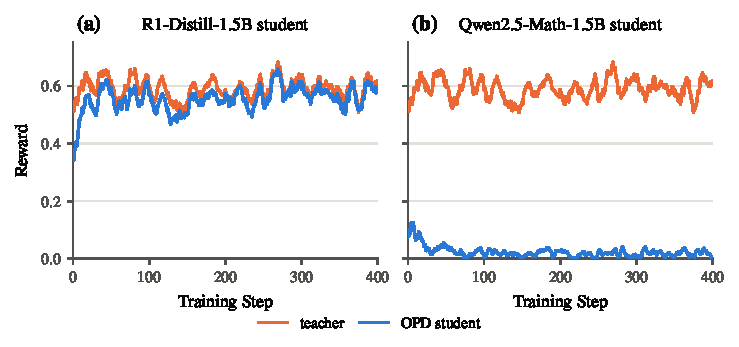
\includegraphics[width=\linewidth]{media/selfdist_distal.pdf}
\caption{Reward curve of distal OPD with the JustRL teacher and two initial students.
OPD rollout correctness increases for R1-Distill-1.5B but decreases
and remains low for Qwen2.5-Math-1.5B. Note that since we do not have student's on policy samples in SFT, we can not draw a similar reward curve for SFT. Their
evaluation results are reported in
Table~\ref{tab:distillation-performance}.}
\label{fig:distillation-distal}
\end{figure}

These results illustrate that successful OPD depends on the
teacher--student pair. They are compatible with the conditional
variance comparison in Appendix~\ref{app:distal-gradient-variance},
but do not identify gradient variance as the cause of the observed
failure. The experiments change the student initialization and do not
measure the teacher-probability suppression condition in
Lemma~\ref{lem:distal-gradient-variance}. Consequently, they do not
establish that a large performance gap alone implies OPD instability.
\FloatBarrier

\clearpage
\subsection{Evaluation results}

\begin{table}[htbp]
\centering
\caption{Evaluation results of OPD and SFT with 16 sampled responses per problem. We can see that OPD typically outperforms SFT in proximal distillation, while it may experience severe instability issue in distal distillation.}
\label{tab:distillation-performance}
\vspace{5pt}
\begingroup
\small
\setlength{\tabcolsep}{5pt}
\renewcommand{\arraystretch}{1.45}
% Match the main table's group headings, spanning all seven columns here.
\newcommand{\distillationgroup}[1]{%
  \specialrule{\lightrulewidth}{2pt}{0pt}%
  \multicolumn{7}{l}{\textcolor{frameworkink}{\textbf{#1}}}\\%
  \specialrule{\lightrulewidth}{0pt}{2pt}}
% Account for the partial rule when vertically centering each four-row cell.
\newcommand{\distillationcell}[2]{%
  \multirow[c]{4}{#1}[-\dimexpr(\aboverulesep+\belowrulesep+\cmidrulewidth)/2\relax]{#2}}
% Shift Teacher left by transferring 8pt of width from Student to its right padding.
  \begin{tabularx}{\linewidth}{>{\raggedright\arraybackslash}X l<{\hspace{14pt}} l r r r r}
\specialrule{\heavyrulewidth}{0pt}{0pt}
\rowcolor{frameworktint}
\textcolor{frameworkink}{\textbf{Student}} &
\textcolor{frameworkink}{\textbf{Teacher}} &
\textcolor{frameworkink}{\textbf{Model}} &
\textcolor{frameworkink}{\textbf{AIME-24}} &
\textcolor{frameworkink}{\textbf{AMC23}} &
\textcolor{frameworkink}{\textbf{MATH500}} &
\textcolor{frameworkink}{\textbf{Mean}} \\
\distillationgroup{Proximal Distillation}
\distillationcell{=}{Qwen3-1.7B-Base} & \distillationcell{*}{GRPO-50} & Student & 0.62 & 7.50 & 16.19 & 8.10 \\
 & & Teacher & 1.04 & 12.19 & 25.62 & 12.95 \\
\cmidrule(l){3-7}
 & & SFT & \textbf{1.88} & \underline{15.78} & \underline{32.69} & \underline{16.78} \\
 & & OPD & \underline{1.25} & \textbf{16.25} & \textbf{35.80} & \textbf{17.77} \\
\midrule
\distillationcell{=}{Qwen3-1.7B-Base} & \distillationcell{*}{GRPO-100} & Student & 0.62 & 7.50 & 16.19 & 8.10 \\
 & & Teacher & \textbf{1.67} & \underline{18.28} & 33.50 & 17.82 \\
\cmidrule(l){3-7}
 & & SFT & \underline{1.04} & \textbf{19.06} & \underline{39.32} & \underline{19.81} \\
 & & OPD & 0.62 & \textbf{19.06} & \textbf{42.58} & \textbf{20.75} \\
\midrule
\distillationcell{=}{Qwen3-1.7B-Base} & \distillationcell{*}{GRPO-200} & Student & 0.62 & 7.50 & 16.19 & 8.10 \\
 & & Teacher & 2.50 & 22.50 & 46.27 & 23.76 \\
\cmidrule(l){3-7}
 & & SFT & \textbf{3.33} & \underline{25.16} & \underline{49.73} & \underline{26.07} \\
 & & OPD & \underline{2.92} & \textbf{25.62} & \textbf{51.36} & \textbf{26.63} \\
\distillationgroup{Distal Distillation}
\distillationcell{=}{R1-Distilled-Qwen-1.5B} & \distillationcell{*}{JustRL-DS} & Student & 21.04 & 63.75 & 75.90 & 53.56 \\
 & & Teacher & \textbf{49.38} & 83.28 & 84.16 & \underline{72.27} \\
\cmidrule(l){3-7}
 & & SFT & \underline{47.92} & \textbf{85.16} & \textbf{85.74} & \textbf{72.94} \\
 & & OPD & 47.29 & \underline{83.44} & \underline{85.39} & 72.04 \\
\midrule
\distillationcell{=}{Qwen2.5-Math-1.5B} & \distillationcell{*}{JustRL-DS} & Student & 4.38 & 18.44 & 23.00 & 15.27 \\
 & & Teacher & \textbf{49.38} & \textbf{83.28} & \textbf{84.16} & \textbf{72.27} \\
\cmidrule(l){3-7}
 & & SFT & \underline{11.88} & \underline{56.09} & \underline{74.41} & \underline{47.46} \\
 & & OPD & -- & -- & -- & -- \\
\bottomrule
\end{tabularx}
\endgroup
\end{table}

Table~\ref{tab:distillation-performance} shows that OPD achieves a
higher mean score than SFT with each of the three nearby teachers.
For R1-Distill-1.5B, both methods attain performance close to the
JustRL teacher, with SFT obtaining the higher mean score. For
Qwen2.5-Math-1.5B, SFT improves the student's mean score from 15.27
to 47.46, while direct OPD fails. The relative effectiveness of the
two objectives therefore varies across teacher--student pairs.

\begin{takeaway}
OPD is favored in the proximal comparisons, consistent with its
local gradient-estimation advantage, while sampled-response KD remains
effective in the larger-gap setting where direct OPD fails.
\end{takeaway}
\FloatBarrier
